\chapter{Parameterbeschaffung}

Zur Bestimmung einer besonders effizienten Strategie um den deutschen Wohngebäudebestand emissionsärmer zu gestalten, wird das in Kapitel \ref{sec:Sektion 32} vorgestellte Optimierungsmodell erweitert.
Hierbei werden in \ref{sec:Sektion 41} die Gebäudeklassen des Bestandes repräsentativ zusammengefasst, um dadurch weniger Optimierungsergebnisse mit geringer Einbuße an Aussagekraft zu erhalten.
Weiterhin wird die Berechnung der Lüftungswärmeverluste des Programms in einen dynamischen Ansatz überführt, um diese genauer abzubilden.
Hierfür werden in \ref{sec:Sektion 42} die Generierung weiterer Daten beschrieben, welche zur dynamischen Modellierung der Wärmeverluste durch Lüftung benötigt werden.

\section{Kategorisierung des Gebäudebestandes}
\label{sec:Sektion 41}

Die Einteilung des deutschen Wohngebäudebestandes nach TABULA sieht 43 Klassen vor, welche die Gebäude nach Baujahr und Gebäudeart unterscheiden.
Dies ist in Tabelle \ref{tab: TabelleA0} zu sehen, aus welcher zudem hervorgeht, dass nicht für alle Baujahre und Gebäudetypen Daten der Wohneinheitenanzahl hinterlegt sind.
Außerdem unterscheiden sich die Anteile der einzelnen Gruppen am gesamten Wohneinheitenbestand.
So bilden beispielsweise die Klasse der Hochhäuser in den alten Bundesländer nur 1\,\% des Bestandes ab, wohingegen der Anteil der Mehrfamilienhäuser 38\,\% beträgt.
Eine einzelne Optimierung aller Gebäudetypen führt zu einer Vielzahl an Ergebnissen, wodurch die Auswertung kompliziert gestaltet wird.

Um aus dieser inhomogenen Verteilung eine vereinfachte Kategorisierung zu gewinnen, werden die Wärmedurchgangskoeffizienten der Gebäudehülle betrachtet.
Neben diesem Kriterium fließen weiterhin die Wohnfläche und die Anzahl der Wohneinheiten der jeweiligen Gebäudetypen mit in die Betrachtung ein.
Da als Ziel dieser Arbeit das Aufweisen von Einsparpotentialen definiert ist, werden Gebäudetypen zusammengefasst, in welchen sich die U-Wert der Gebäudehülle gleichen.

Zunächst werden die Einfamilienhäuser mit den Reihenhäusern verglichen.
Diese Gebäudetypen besitzen beiden zwischen 1 bis 2 Wohnungen.
Die Wohnflächen der Einfamilienhäuser betragen für die TABULA-Referenzgebäude zwischen 100 bis 200\,m\(^2\) und die der Reihenhäuser zwischen 90 und 130\,m\(^2\).\\
Bis auf wenige Ausnahmen gleichen sich die U-Werte der Einfamilien- und Reihenhäuser.
Solch eine Ausnahme wird bei den Fenstern der Altersgruppe mit Baujahr von 1979 bis 1983 gefunden.
Den Einbaustandard in den Einfamilienhäusern dieser Jahrgänge bildet die Zweischeiben-Verglasung mit Metallrahmen.
Aufgrund dessen schlechten Wärmeübertragungsverhaltens besitzt die Verglasung der Einfamilienhäuser der Baualtersklasse von 1979 bis 1983 einen U\(_w\)-Wert in Höhe von 4,3 \(\frac{W}{m^2 \cdot K}\).
Im Vergleich dazu liegt bei den Reihenhäuser derselben Jahrgänge mit gleicher Verglasung jedoch mit Holzrahmen anstelle des Metallrahmens ein U\(_w\)-Wert von 2,8 \(\frac{W}{m^2 \cdot K}\) vor.\\
Weiterhin weichen die Wärmedurchgangskoeffizienten der Dächer für die Baualtersklassen von 1860 bis 1968 voneinander ab.
Der U-Wert des Referenzgebäudes bewegt sich in diesem Zeitraum zwischen 1,4 und 0,8 \(\frac{W}{m^2 \cdot K}\), wohingegen dieser bei den Reihenhäusern mit Werten zwischen 1,0 und 0,6 \(\frac{W}{m^2 \cdot K}\) leicht besser vorliegt.\\
Da bis auf die zwei erläuterten Unterschiede die U-Werte nahezu identisch vorliegen, werden die Gebäudetypen der Einfamilien- und Reihenhäuser zusammengefasst.
Durch lineare Interpolation der unterschiedlichen U-Werte anhand der Wohneinheitenanzahl der jeweiligen Gebäudetypen, wird der Einfluss der besseren Wärmedämmung beachtet.\\
Die aus den Einfamilien- und Reihenhäuser neu entstandene Gruppe wird im Weiteren als \mbox{\textit{Cluster A}} bezeichnet. \cite{.2015}

Als nächstes werden die Mehrfamilienhäuser mit der Klasse der großen Mehrfamilienhäuser in den neuen und alten Bundesländer verglichen.
Betrachtet man hier zunächst die Wärmedurchgangskoeffizienten der Gebäudehülle, lassen sich nur vereinzelt leichte Unterschiede festmachen.
So unterscheidet sich beispielsweise der Wärmedurchgang durch die Außenwand in den Jahren 1979 bis 1983 zwischen dem Gebäudetyp der Mehrfamilienhäuser und dem der großen Mehrfamilienhäuser in den neuen Bundesländern um eine Differenz von 0,1 \(\frac{W}{m^2 \cdot K}\) und somit 11\,\%. \\
Hinsichtlich der Wohnfläche je Wohnung und der Wohnungsanzahl variieren die drei Gebäudetypen der Mehrfamilienhäuser.
Allerdings unterscheiden sich diese Faktoren auch innerhalb des Gebäudetyps der Mehrfamilienhäuser.
So definiert TABULA als Referenzgebäude der Mehrfamilienhäuser der Jahrgänge 1949 bis 1957 ein dreigeschossiges Wohngebäude mit 9 Wohnungen und 575\,m\(^2\) beheizter Wohnfläche. 
Die darauffolgende Altersklasse von 1958 bis 1968 desselben Gebäudetypes wird durch ein viergeschossiges Wohngebäude mit 32 Wohnungen und 2845\,m\(^2\) beheizter Wohnfläche beschrieben.
Um die Gebäudetypen der Mehrfamilienhäuser und der großen Mehrfamilienhäuser in den neuen und alten Bundesländer zusammenzufassen, werden die Wohnfläche sowie die Faktoren zur Bestimmung der Dach-, Außenwand-, Fenster- und Bodenfläche anhand der Wohneinheitenanzahl linear interpoliert.
Dadurch wird eine neue Klasse generiert, welche im Folgenden mit \mbox{\textit{Cluster B}} bezeichnet wird.

In Tabelle \ref{tab: TabelleA0} sind außer den nun in Cluster A und Cluster B integrierten Gebäudetypen noch Hochhäuser in den neuen und alten Bundesländer zu finden.
Deren Anteil an allen Wohneinheiten in Deutschland beträgt weniger als 2\,\%. 
Außerdem ist deren Wohnfläche und Wohnungsanzahl je Gebäude um ein Vielfaches größer als die der Mehrfamilienhäuser.
Somit sind die Hochhäuser zur Betrachtung eines energetischen Einsparpotenzials weniger relevant und werden nicht weiter berücksichtigt.

Im Bezug auf die Baujahre lassen sich ebenfalls Jahrgänge mit ähnlichen energetischen Eigenschaften der Gebäudehülle erkennen.
Auf eine Betrachtung von Wohngebäuden mit Baujahr älter als 1860 wird verzichtet, da diese zum einen keinen relevanten Anteil am Bestand besitzen und zum anderen deren U-Werte stark von der darauffolgenden Baualtersklasse abweichen.\\
Weiterhin werden Gebäude mit einem Neubau-Standard nach der 3. WschV vernächlassigt.
Zwar handelt es sich hierbei um Gebäude, welche mitunter 25 Jahre alt sind und somit Sanierungsbedarf besteht, jedoch bergen diese Wohngebäude aufgrund der relativ guten energetischen Bauweisen ein geringes Einsparpotential an CO\(_2\).

Nach Eicke-Henning \cite{EickeHenning.2011} und Tabelle \ref{tab: TabelleA0} weisen die U-Werte der Bauteile mit Jahrgang 1860 bis 1957 aufgrund ähnliche Baustoffe und Bauweisen Gemeinsamkeiten auf.
Nach 1957 verbessern sich diese bis zur 1. WschV 1978 aufgrund der Wahl anderer Baustoffe und dem technologischem Fortschritt im Hochbau.
Im Zuge der 1. und 2. WschV lassen sich Verbesserungen der energetischen Qualität der Hülle im Zeitraum von 1978 bis 1994 erkennen.
Somit werden die Jahrgänge von 1860 bis 1994 in drei Epochen unterteilt.
Die älteste Epoche umfasst alle Baujahre inklusive der Nachkriegszeit und daher 1860 - 1957.
Die nächste beschreibt die Jahrgänge von 1958 bis 1978 und beinhaltet somit den Zeitraum nach der Nachkriegszeit, in der ohne Regulation durch den Gesetzgeber die Gebäudehülle verbessert wurde.
Zuletzt charakterisiert die dritte Epoche von 1979 bis 1994 Bauten mit Baustandard der 1. und 2. WschV.\\
Zur Bestimmung der U-Werte der neu generierten Klassen werden die Wärmedurchgangskoeffizienten der ursprünglichen Gebäudetypen auf Basis ihrer Wohneinheitenanzahl linear interpoliert.
In Tabelle \ref{tab: TabelleA411} sind die neuen Klassen mitsamt der jeweiligen U-Werte der Hüllenbestandteile aufgeführt.

\begin{table}[H]\centering
\begin{tabular}{|l|l|c|c|c|}
\hline
\rowcolor[HTML]{9B9B9B} 
\cellcolor[HTML]{9B9B9B} & \cellcolor[HTML]{9B9B9B} & \multicolumn{3}{c|}{\cellcolor[HTML]{9B9B9B}Baualtersklasse} \\ \cline{3-5} 
\rowcolor[HTML]{9B9B9B} 
\multirow{-2}{*}{\cellcolor[HTML]{9B9B9B}Gebäudetyp} & \multirow{-2}{*}{\cellcolor[HTML]{9B9B9B}Bauteil} & \multicolumn{1}{l|}{\cellcolor[HTML]{9B9B9B}\begin{tabular}[c]{@{}l@{}}1856\\ -1957\end{tabular}} & \multicolumn{1}{l|}{\cellcolor[HTML]{9B9B9B}\begin{tabular}[c]{@{}l@{}}1957\\ -1978\end{tabular}} & \multicolumn{1}{l|}{\cellcolor[HTML]{9B9B9B}\begin{tabular}[c]{@{}l@{}}1979\\ -1994\end{tabular}} \\ \hline
\cellcolor[HTML]{c0c0c0} & Dach & 1,29 & 0,64 & 0,43 \\ \cline{2-5} 
\rowcolor[HTML]{EFEFEF} 
\cellcolor[HTML]{c0c0c0} & Außenwand & 1,59 & 1,1 & 0,61 \\ \cline{2-5} 
\cellcolor[HTML]{c0c0c0} & Fenster & 2,8 & 2,8 & 2,8 \\ \cline{2-5} 
\rowcolor[HTML]{EFEFEF} 
\multirow{-4}{*}{\cellcolor[HTML]{c0c0c0}Cluster A} & Boden & 0,82 & 0,93 & 0,56 \\ \hline
\cellcolor[HTML]{c0c0c0} & Dach & 1,24 & 0,51 & 0,39 \\ \cline{2-5} 
\rowcolor[HTML]{EFEFEF} 
\cellcolor[HTML]{c0c0c0} & Außenwand & 1,61 & 1,11 & 0,68 \\ \cline{2-5} 
\cellcolor[HTML]{c0c0c0} & Fenster & 3 & 3 & 3 \\ \cline{2-5} 
\rowcolor[HTML]{EFEFEF} 
\multirow{-4}{*}{\cellcolor[HTML]{c0c0c0}Cluster B} & Boden & 1,03 & 0,93 & 0,56 \\ \hline
\end{tabular}
\caption{U-Werte der neuen Gebäudeklassen Cluster A und Cluster B in \(\frac{W}{m^2 \cdot K}\)}
\label{tab: TabelleA411}
\end{table}

\section{Parameter zur Modellierung von Lüftungswärmeverlusten}
\label{sec:Sektion 42}

Aus der Darstellung der Lüftungswärmeverluste in Kapitel \ref{sec:Sektion 33} geht hervor, dass diese zum einen vom Lüftungsverhalten der Bewohner und zum anderen durch thermische und Wind abhängige Triebkräfte charakterisiert werden.
Diese Faktoren werden in dem zu Grunde liegenden Optimierungsprogramm nicht abgebildet, weshalb das Programm um diese Einflussfaktoren erweitert wird.
Zur besseren Abbildung des Nutzereinflusses werden zunächst Fensteröffnungsprofile erstellt.

Um das Nutzerverhalten bezüglich der Fensterlüftung zu modellieren, werden Parameter, welche den Bewohner animieren ein Fenster zu öffnen oder zu schließen, festgelegt.
Nach Calí et al. beeinflussen den Nutzer die Tageszeit, die CO\(_2\)-Konzentration im Raum, die Innen- und Außentemperatur sowie die Luftfeuchtigkeit im Inneren des Gebäudes und der Umgebung (s. Tabelle \ref{tab: Tabelle3312}).
Da im Rahmen dieses Optimierungsprogramms weder Kohlenstoffdioxid noch Luftfeuchtigkeit modelliert werden, können diese Einflussfaktoren nicht abgebildet werden.
Weiterhin wird eine konstant bleibende Innentemperatur von 20°C angenommen, weswegen die Raumtemperatur auch als Einflussfaktor keine Berücksichtigung findet.
Somit verbleiben die Tageszeit und die Außentemperatur als relevante Faktoren, welche den Nutzereinfluss auf die Lüftungswärmeverluste beschreiben.

Als Grundlage der Fensteröffnungsprofile dienen die Monitoring-Daten eines Forschungsprojekts an drei Mehrfamilienhäusern in Karlsruhe-Rintheim.
Bei diesem Projekt wurden die Auswirkungen von Sanierungsmaßnahmen und unterschiedlicher Anlagentechnik auf den Energieverbrauch analysiert.
Die drei Häusern sind in jeweils drei Riegel unterteilt, in welchen sich jeweils 10 Wohnungen mit je 72 m\(^2\) befinden.
Die vorgenommenen Sanierungsmaßnahmen und die genutzte Anlagentechnik inklusive der Lüftungskonzepte sind Tabelle AXXXX zu entnehmen.
Da nach Osterhage \cite{Osterhage.2018} kein signifikanter Unterschied des Nutzerverhaltens in den Wohnungen mit maschinellen Lüftungsanlagen im Vergleich zu denen mit freier Lüftung besteht, werden die Daten aller Wohnungen in Betracht gezogen.

An zwei der drei Untersuchungsobjekte wurden Daten des Fensterzustandes und der Außentemperatur erhoben.
Bei diesen handelt es sich um minütlich aufgezeichnete Binärvariablen, welche pro Fenster und Wohnung angeben, ob das Fenster zu dem Zeitpunkt offen (1) oder geschlossen (0) ist.
Als Ziel der Fensteröffnungsprofile werden Tagesprofile des Fensteröggnungsverhalten der Bewohner mit einer Temperatur- und Tageszeitabhängigkeit definiert.

Aufgrund der deutlich höheren Rechendauer einer minütlichen Betrachtung, werden zunächst die Werte in stündliche umgewandelt. 
Hierfür wird je Fenster das arithmetische Mittel einer Stunde gebildet.
Die Variable wird hierbei nicht weiter als Binärvariable angenommen, sondern als Dauer betrachtet.
Hierbei bedeutet eine 1, dass das Fenster eine Minute lang geöffnet ist.
Das Ergebnis dieses Rechenschritts ist keine Binärvariable, sondern eine reelle Zahl zwischen 0 und 1, welche die Öffnungsdauer des Fensters zu jedem stündlichen Zeitpunkt des Jahres beschreibt.
Beispielsweise wird durch den Wert 0,5 beschrieben, dass das Fenster in der betrachteten Stunde 30 Minuten geöffnet ist.\\
Im nächsten Schritt werden die Fenster der Wohnung zusammengefasst.
Wie in \cite{Osterhage.2018} beschrieben, werden die Räume je nach Nutzung unterschiedlich belüftet.
Da in dem Referenzmodell jedoch keine Unterteilung in Räume geschieht, werden die Fensteröffnungszeiten auf Wohnungsebene betrachtet.
Hierzu werden die Öffnungsdauern aller Fenster einer Wohnung je Stunde aufsummiert.
Die daraus erhaltene Größe ist rein hypothetisch und kann als Dauer einer unbekannten Menge an geöffneten Fenster interpretiert werden.
Als Beispiel sagt der Wert 1 aus, dass ein Fenster die ganze Stunde geöffnet ist oder aber zwei Fenster jeweils eine halbe Stunde.
Da von Fenstern mit gleicher Geometrie und nur einem möglichen Öffnungswinkel ausgegangen wird, gibt es zwischen den zwei Beispielfällen keinen Unterschied im Bezug auf die Lüftungswärmeverluste.
Das Ergebnis dieser Rechenschritte beschreibt stundenweise Fensteröffnungsprofile einer Wohnung, die über ein Jahr aufgetragen sind.\\
Die stündlichen Werte werden über alle Wohnungen des Datensatzes gemittelt.
Somit wird aus den 60 Wohnungen des Forschungsprojekts ein Jahresprofil erzeugt, welches die Öffnungsdauer einer unbekannten Menge an Fenstern je Stunde des Jahres beschreibt.
Um sowohl die Außentemperatur als auch die Tageszeit in den Fensteröffnungsprofilen zu berücksichtigen, werden Temperaturintervalle mit ähnlichem Nutzerverhalten gebildet. 
Bei ähnlichen Außentemperaturen zeigt das Lüftungsverhalten der Bewohner Gemeinsamkeiten unabhängig der Jahreszeit \cite{Osterhage.2018}.
Temperaturen kleiner \mbox{0°C} werden mit dem Temperaturintervall \mbox{-5°C} und dem Intervall \mbox{[-5°C, 0°C)} abgebildet.
Für Temperaturen größer als \mbox{0°C} werden die Intervalle in 3\,K Schritten bis \mbox{15°C} gebildet und somit die Intervalle \mbox{[0°C, 3°C)}, \mbox{[3°C, 6°C)}, \mbox{[6°C, 9°C)}, \mbox{[9°C, 12°C)} und \mbox{[12°C, 15°C)} festgelegt.
Für Tage, an welchen sich die durchschnittliche Tagestemperatur in demselben Temperaturintervall befindet, werden die hypothetischen Fensteröffnungsdauern je Tageszeitpunkt gemittelt.
Somit werden Tagesprofile der Fensteröffnungszeiten für unterschiedliche Temperaturintervalle einer Wohnung erzeugt.
In Abbildung \ref{fig: Abbildung421} sind exemplarische Fensteröffnungsprofile der Temperaturintervalle [9,12) und [12,15) dargestellt.

\begin{figure}[H]
	\centering
		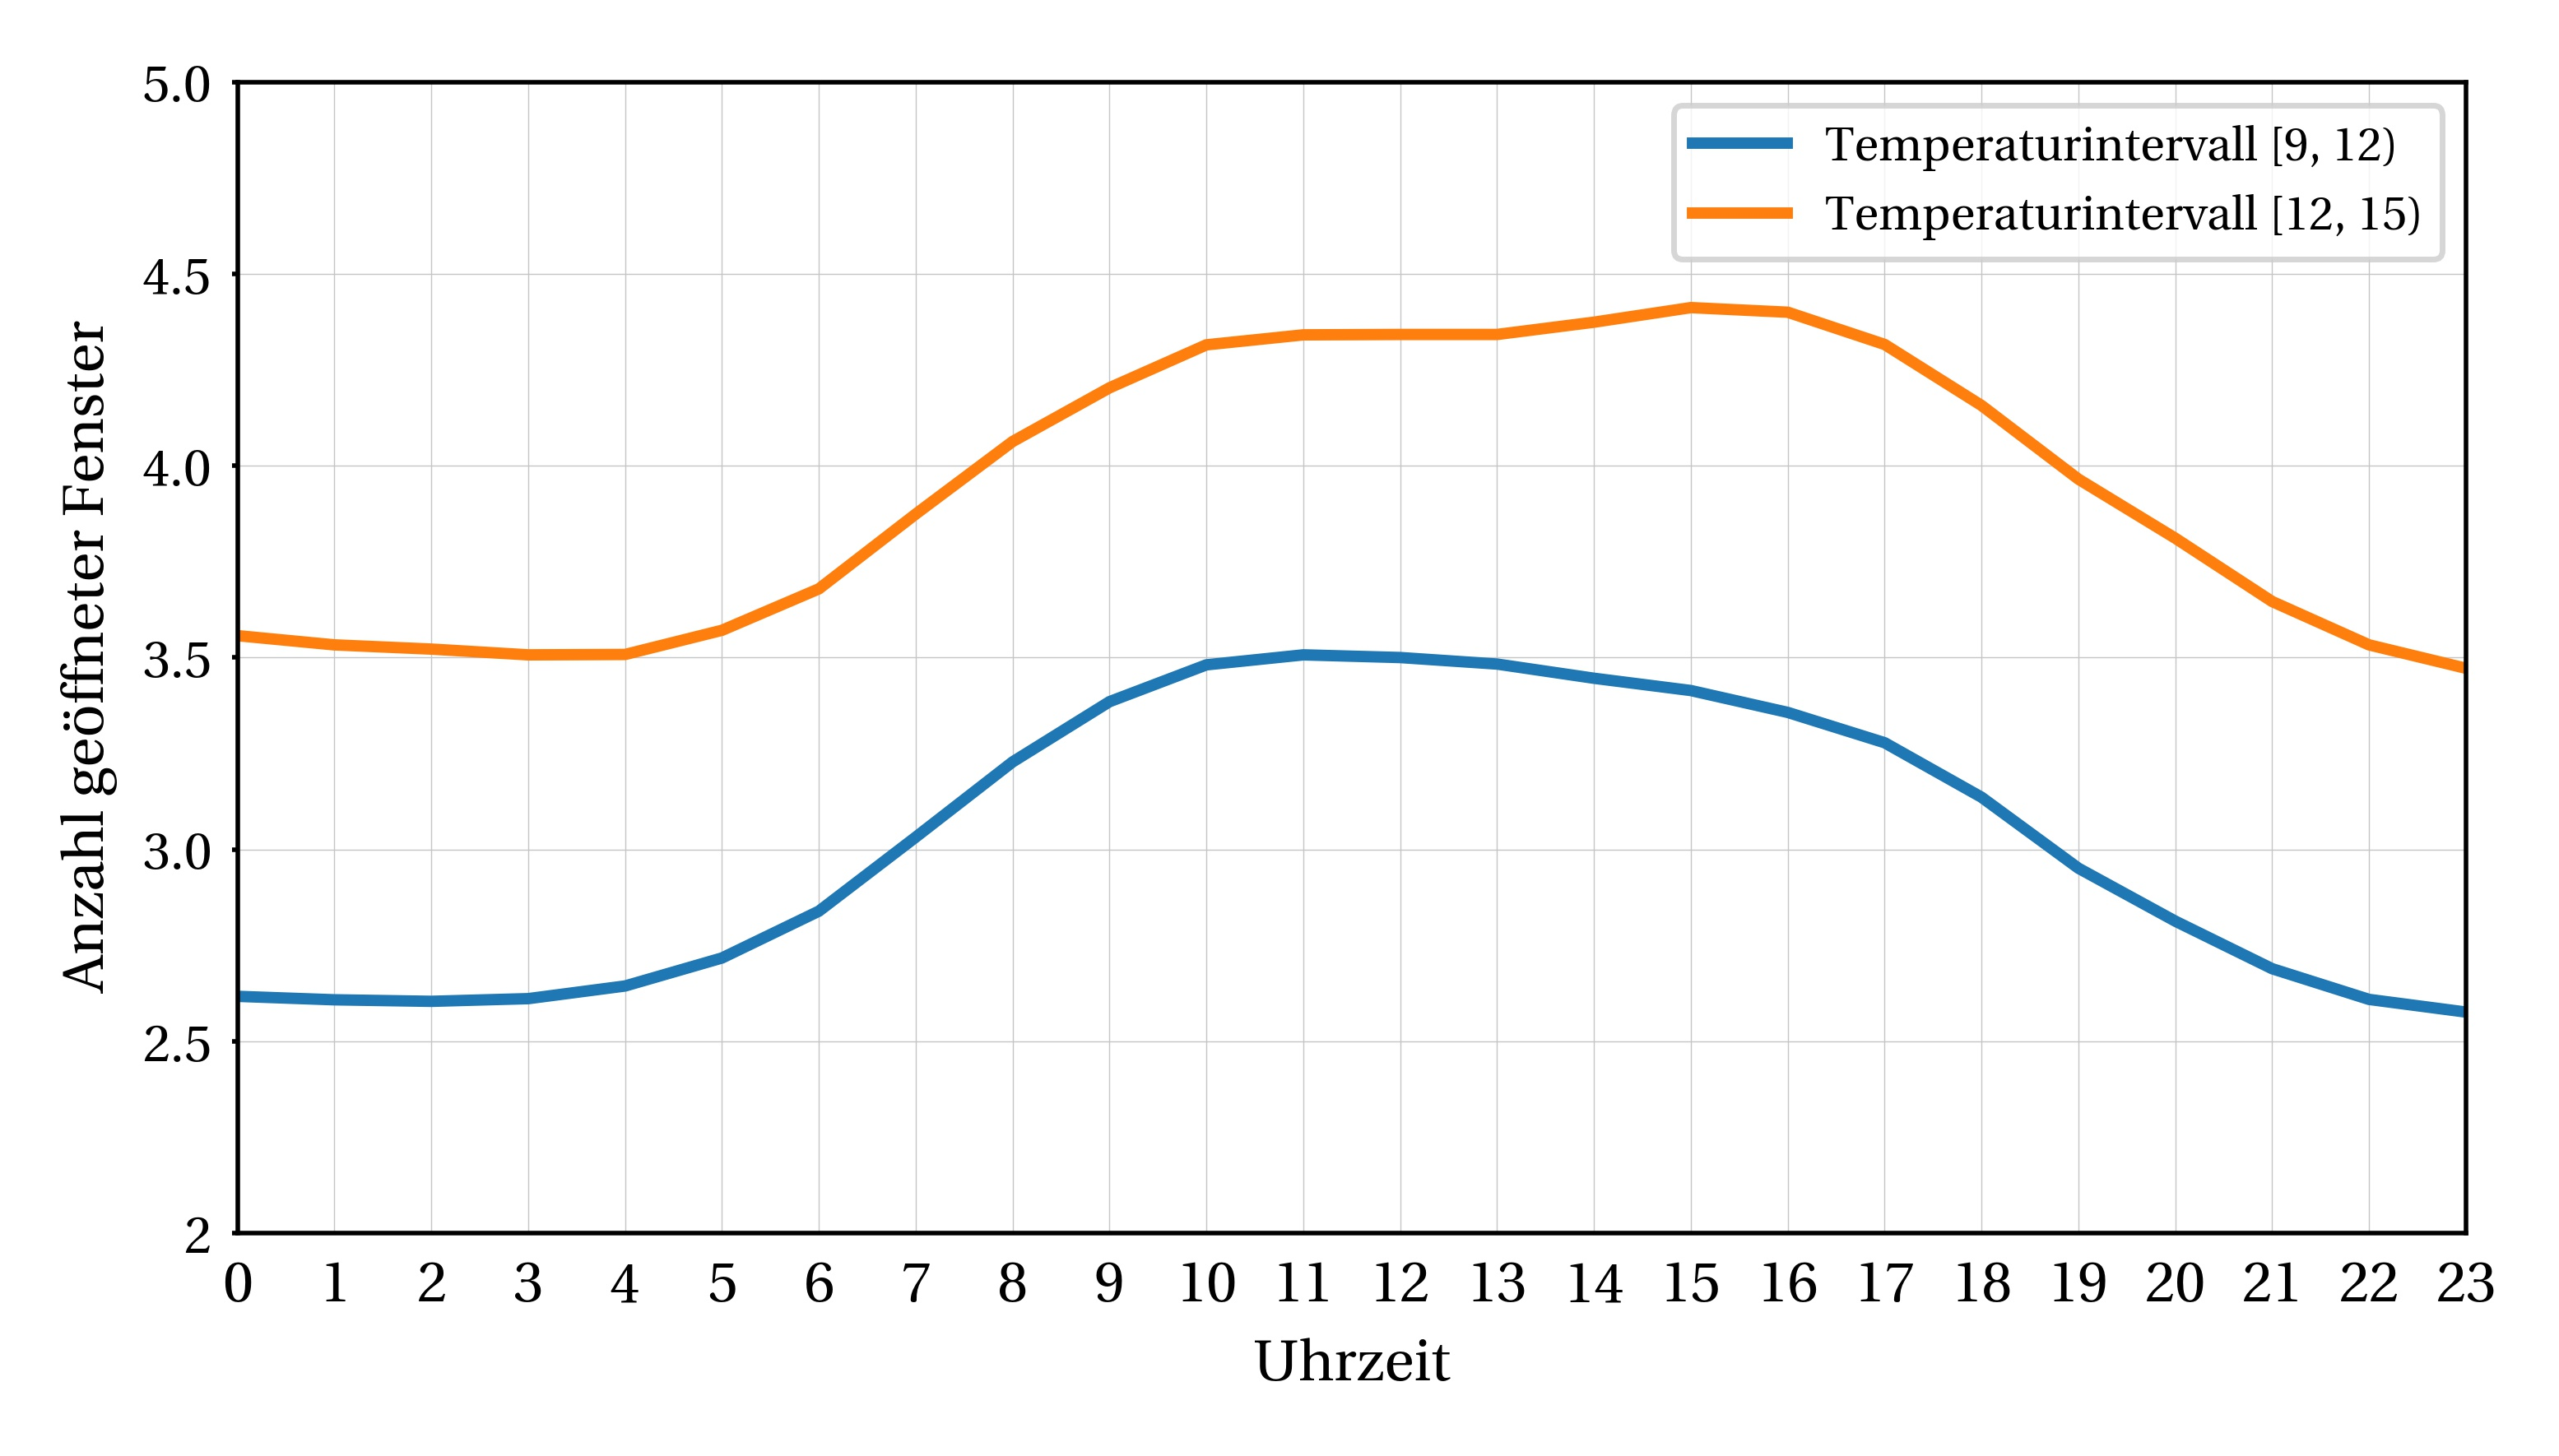
\includegraphics{Pictures/Fensteroeffnungsprofile.jpg}
	\caption{tba}
	\label{fig: Abbildung421} 
\end{figure}

Neben dem geöffneten oder geschlossenen Zustand eines Fensters beeinflussen die Temperaturdifferenz zwischen Innen- und Außentemperatur sowie die Windgeschwindigkeit den durch ein Fenster einströmenden Luftvolumenstrom.
Die Temperaturdifferenz kann durch Temperaturprofile gebildet werden, welche bereits in das Optimierungsprogramm eingelesen werden.
Zur Bestimmung von Profilen der Windgeschwindigkeit werden die Daten des Deutschen Wetterdienstes für das Testreferenzjahr genutzt \cite{try}.
Diese umfassen unter anderem die Windgeschwindigkeit in 10\,m Höhe für 15 verschiedene Klimaregionen in Deutschland.
Diese Klimaregionen werden durch eine Repräsentanzstation vertreten, welche den möglichen Gebäudelagen des Optimierungsprogramms entsprechen (s. Tabelle \ref{tab: TabelleA4}.
Somit werden für die jeweiligen Standorte Profile des Windes in 10\,m Höhe für 8760 Zeitpunkte eines Jahres generiert.









